\documentclass[11pt]{article}
\usepackage[margin=1in]{geometry}
\usepackage{amsmath,amssymb,graphicx,xcolor}
\usepackage[hidelinks]{hyperref}
\usepackage{caption}
\captionsetup{font=small,labelfont=bf}
\graphicspath{{figures/}}
\newcommand{\msun}{M_\odot}
\newcommand{\az}{a_0}
\newcommand{\gext}{g_{\rm ext}}
\newcommand{\gbar}{g_{\rm bar}}
\newcommand{\Ez}{E(z)}

\title{\bf A redshift-dependent External Field Effect as a decisive test of an
evolving MOND scale:\\ forecast and observing proposal}
\author{Carl Zimmerman\\[2pt]
\small\it with computational review support}
\date{June 2026}

\begin{document}
\maketitle

\begin{abstract}
\noindent
The Milgromian acceleration scale $\az\simeq1.2\times10^{-10}\,{\rm m\,s^{-2}}$ is
numerically close to the cosmic acceleration $cH_0$. If this is causal rather than
coincidental---$\az=\tfrac{c}{2}\sqrt{G\rho}=cH(z)/Z$, so that the scale tracks the
mean cosmic density---then $\az$ \emph{evolves}, $\az(z)=\az(0)\Ez$ with
$\Ez=\sqrt{\Omega_m(1+z)^3+\Omega_\Lambda}$. We point out that this hypothesis makes
one prediction that is both \emph{forbidden in $\Lambda$CDM} and \emph{distinct from
constant-$\az$ MOND}: the External Field Effect (EFE) must weaken with redshift, its
strength scaling as $\eta(z)=\gext/\az(z)=\eta_0/\Ez$. We compute the observable
signal (the change in the embedded-versus-isolated mass-discrepancy offset, $\sim
0.1$\,dex out to $z\simeq4$--$6$), build an honest per-galaxy error budget
($\sigma\simeq0.25$--$0.41$\,dex), and derive the required sample: $\sim$590
(optimistic) to $\sim$1600 (realistic) \emph{extended, environment-resolved}
galaxies with kinematics, baryonic masses and a measured external field, the
discriminating power concentrated at $z\gtrsim2$. We lay out a concrete, staged
JWST\,+\,ALMA\,+\,ELT campaign. We are explicit that the present direct evidence for
$\az(z)$ is only a $\sim2\sigma$, single-point-driven, $\Lambda$CDM-degenerate hint;
the EFE-evolution test is the cleaner discriminator and a next-decade measurement.
\end{abstract}

\section{Introduction}
Modified Newtonian Dynamics (MOND; \cite{Milgrom1983,Famaey2012}) organises galaxy
dynamics around a single acceleration scale $\az$: where the gravitational
acceleration falls below $\az$, the observed acceleration $g_{\rm obs}$ exceeds the
Newtonian baryonic value $\gbar$, following the radial acceleration relation (RAR)
with remarkably small scatter \cite{McGaugh2016,Lelli2017}. The value of $\az$ has a
famous numerical property: $2\pi\az\approx cH_0\approx c^2\sqrt{\Lambda/3}$. Two
readings are possible---$\az$ is a new fundamental constant, or it is set by
cosmology \cite{Milgrom2011,Milgrom2014}. We take the second, in the specific form
\begin{equation}
\az \;=\; \frac{c}{2}\sqrt{G\rho}\;=\;\frac{cH(z)}{Z},\qquad Z=2\sqrt{8\pi/3}\simeq5.79,
\label{eq:law}
\end{equation}
where the second equality uses the Friedmann relation $H^2=\tfrac{8\pi G}{3}\rho$.
Reading $\rho$ as the cosmic mean density makes $\az$ a function of epoch:
\begin{equation}
\az(z)=\az(0)\,\Ez,\qquad \Ez=\sqrt{\Omega_m(1+z)^3+\Omega_\Lambda}.
\label{eq:evol}
\end{equation}
The evolving-scale idea is Milgrom's \cite{Milgrom2014}; what we contribute here is a
single \emph{clean, falsifiable} consequence and the survey design to test it. That
consequence lives in the MOND External Field Effect.

\paragraph{The External Field Effect.}
MOND is nonlinear in acceleration, so---unlike Newtonian gravity or particle dark
matter, which obey the strong equivalence principle---a \emph{uniform external field}
$\gext$ alters a system's internal dynamics \cite{BekensteinMilgrom1984}. The
controlling ratio is $\eta\equiv\gext/\az$: when $\eta\gtrsim1$ the external field
drives the system toward the Newtonian regime and the MOND boost is suppressed; when
$\eta\ll1$ the system is in isolated, deep-MOND. The EFE is arguably detected at
$z\simeq0$ in the outer rotation curves of SPARC galaxies \cite{Chae2020}, though the
significance is debated. Our point is simple: in Eq.~(\ref{eq:evol}) the
\emph{denominator} of $\eta$ grows with redshift, so
\begin{equation}
\boxed{\;\eta(z)=\frac{\gext}{\az(z)}=\frac{\eta_0}{\Ez}\;}
\label{eq:efe}
\end{equation}
and the EFE must \emph{weaken} toward high $z$: at fixed external field, distant
galaxies are more isolated-MOND than their local analogues.

\section{The prediction and what it separates}
Figure~\ref{fig:pred} shows Eqs.~(\ref{eq:evol})--(\ref{eq:efe}). By $z=4$, $\Ez=6.3$,
so a given external environment is $\sim6\times$ less effective at suppressing MOND
than today. Three hypotheses make qualitatively different statements about the
embedded-minus-isolated offset in the mass discrepancy, $\Delta\equiv
\log_{10}(\text{boost}_{\rm emb}/\text{boost}_{\rm iso})$, as a function of redshift:
\begin{itemize}\itemsep1pt
\item \textbf{$\Lambda$CDM / dark matter:} $\Delta(z)=0$ at all $z$ (no EFE; the
equivalence principle holds for internal dynamics).
\item \textbf{Constant-$\az$ MOND:} $\Delta(z)=\text{const}\neq0$ (EFE present, not
evolving).
\item \textbf{Evolving $\az$ (this work):} $\Delta(z)\to0$ as $z$ grows, tracking
$\eta_0/\Ez$.
\end{itemize}
This is the key virtue of the test: the \emph{existence} of a nonzero $\Delta$
already discriminates MOND from dark matter, and its \emph{redshift trend}
discriminates evolving from constant $\az$. Because the EFE is forbidden in
$\Lambda$CDM, the redshift trend cannot be mimicked by halo evolution---the principal
degeneracy that afflicts a direct $\az(z)$ measurement (\S\ref{sec:current}).
Figure~\ref{fig:disc} shows the three curves with forecast error bars.

\begin{figure}[t]
\centering
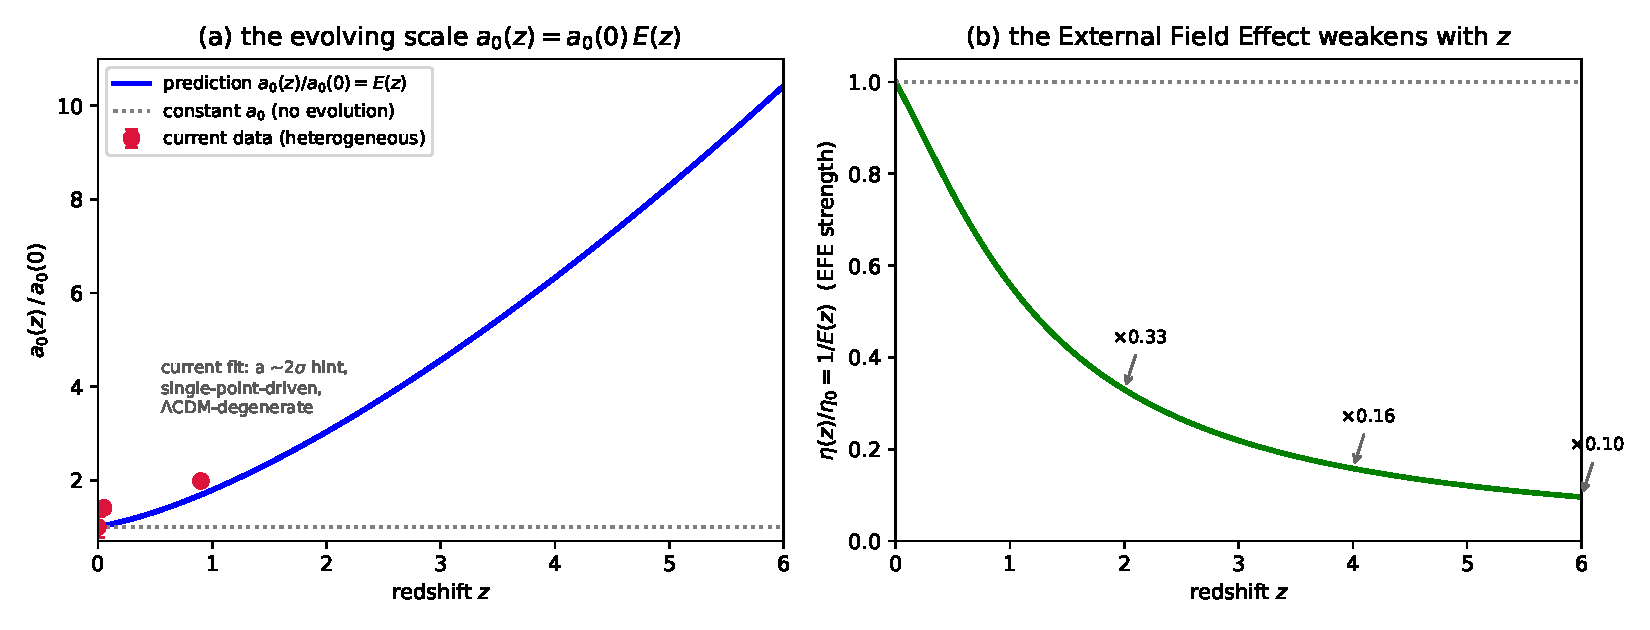
\includegraphics[width=\textwidth]{efe_fig1_prediction.pdf}
\caption{\textbf{The prediction.} (a) The evolving scale $\az(z)=\az(0)\Ez$ (blue),
with the three heterogeneous determinations compiled to date (red; Table~1); the
dotted line is a non-evolving $\az$. (b) The EFE strength $\eta(z)/\eta_0=1/\Ez$: the
external field becomes $\sim3\times$, $6\times$, $10\times$ less effective by
$z=2,4,6$.}
\label{fig:pred}
\end{figure}

\section{The observable}
For a galaxy of baryonic acceleration $\gbar$ in an external field $\gext$, the
algebraic (single-field) MOND/AQUAL prescription with interpolation function
$\mu(x)=x/(1+x)$ gives the internal acceleration $g_{\rm obs}$ by solving
\begin{equation}
\mu\!\left(\frac{g_{\rm obs}+\gext}{\az(z)}\right)g_{\rm obs}=\gbar .
\label{eq:solve}
\end{equation}
The isolated limit ($\gext=0$) recovers $g_{\rm obs}=\sqrt{\gbar\,\az}$; a strong
external field Newtonises the system, $g_{\rm obs}\to\gbar/\mu(\gext/\az)$. The
observable offset is $\Delta(z)=\log_{10}\!\big[(g_{\rm obs}^{\rm emb}/\gbar)/(g_{\rm
obs}^{\rm iso}/\gbar)\big]$. For a deep-MOND galaxy ($\gbar=0.1\,\az$) in a moderate
field ($\gext=0.5\,\az$), Eq.~(\ref{eq:solve}) yields $\Delta=-0.196$\,dex at $z=0$,
rising to $-0.115$\,dex at $z=4$; the full $z=0\to6$ swing for $\gext=\az$ is
$\approx0.12$\,dex (Fig.~\ref{fig:disc}). \emph{This is the signal}---small, but with
a fixed sign and a fixed redshift shape set entirely by $\Ez$.

\section{Current evidence, stated honestly}
\label{sec:current}
Table~1 collects the three published acceleration-scale determinations spanning
cosmic time. A power-law fit $\az\propto(1+z)^p$ gives $p=0.80\pm0.17$, and a constant
$\az$ is nominally disfavoured at $\sim5\sigma$. We do not believe that number. It
rests on a single long-lever-arm point ($z\simeq0.9$), it assumes three
\emph{heterogeneous} measurements (local disk rotation curves; an intermediate
compilation; high-$z$ integral-field dispersions) are commensurate to their small
quoted errors, and folding in the inter-method systematic that the local pair already
demands drops the rejection to $\sim2\sigma$; removing the $z\simeq0.9$ point drops it
to $\sim1.2\sigma$. Moreover a rising \emph{apparent} $\az$ is exactly what
$\Lambda$CDM produces through denser high-$z$ halos and more compact baryons
\cite{Tian2022,deGraaff2024}, so three points cannot separate fundamental $\az(z)$
from astrophysics plus selection. \textbf{The honest status of the direct evidence is
a $\sim2\sigma$ hint in the predicted direction---not a detection.} This is precisely
why the EFE-evolution test matters: it is the same physics seen through a window
($\Delta\neq0$) that dark matter cannot enter.

\begin{table}[h]
\centering
\small
\begin{tabular}{ccl}
\hline
$z$ & $\az\;[10^{-10}\,{\rm m\,s^{-2}}]$ & source \\
\hline
$0.00$ & $1.20\pm0.26$ & SPARC---McGaugh, Lelli \& Schombert 2016 \cite{McGaugh2016}\\
$0.05$ & $1.69\pm0.13$ & V\u{a}r\u{a}\c{s}teanu \textit{et al.} 2025 \cite{Varasteanu2025}\\
$0.90$ & $2.38\pm0.11$ & MUSE--DARK III 2026 \cite{MUSEDARK2026}\\
\hline
\end{tabular}
\caption{The three acceleration-scale determinations used in Fig.~\ref{fig:pred}.
They are heterogeneous in method and sample; the apparent rise is a $\sim2\sigma$
hint, $\Lambda$CDM-degenerate.}
\end{table}

\begin{figure}[t]
\centering
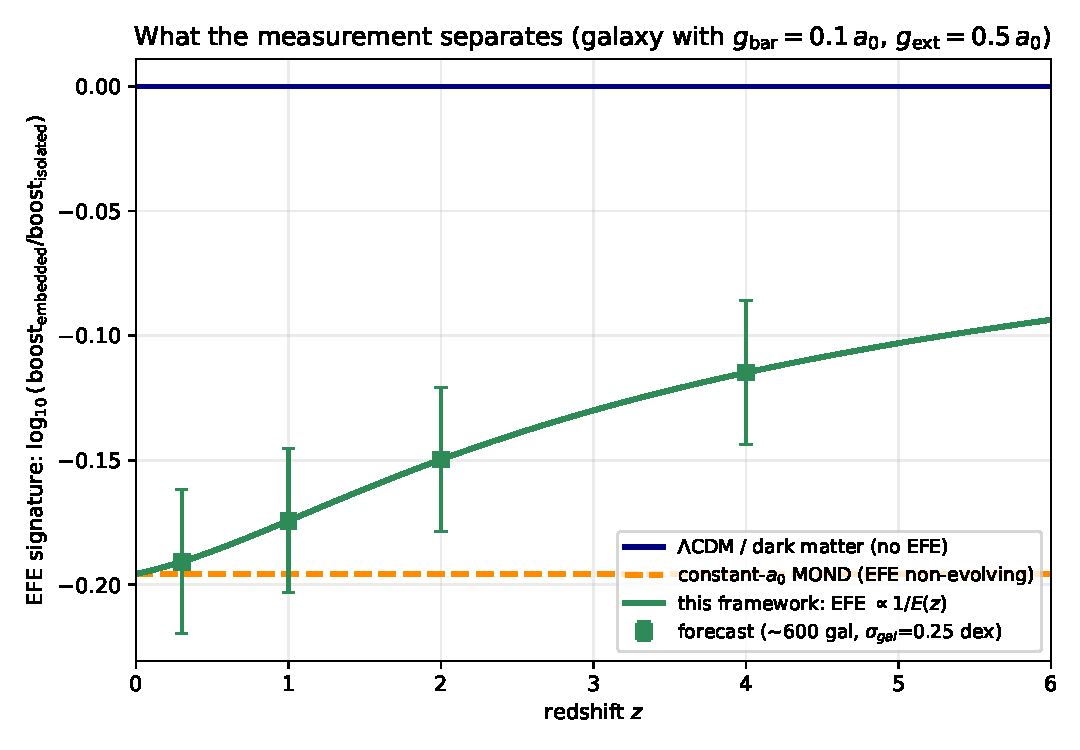
\includegraphics[width=0.74\textwidth]{efe_fig2_discrimination.pdf}
\caption{\textbf{What the measurement separates.} The embedded$-$isolated offset
$\Delta(z)$ for a deep-MOND galaxy. $\Lambda$CDM predicts $\Delta=0$ (no EFE);
constant-$\az$ MOND predicts a non-evolving offset (dashed); the evolving-$\az$
hypothesis predicts $\Delta\to0$ as $\eta_0/\Ez$ (green). Points: forecast for a
$\sim$600-galaxy, $\sigma_{\rm gal}=0.25$\,dex campaign.}
\label{fig:disc}
\end{figure}

\section{Forecast: signal, noise, sample size}
\paragraph{Error budget.} The per-galaxy uncertainty on $\log_{10}(M_{\rm
dyn}/M_{\rm bar})$ at $z>4$ is dominated by (i) dynamical mass from resolved
kinematics ($\sim0.20$\,dex), (ii) stellar mass from SED fitting ($\sim0.25$\,dex;
IMF, SFH, dust), (iii) gas mass, which can dominate the baryons and is rarely measured
($\sim0.20$\,dex), and (iv) the irreducible RAR scatter ($\sim0.15$\,dex). In
quadrature, $\sigma_{\rm gal}\simeq0.41$\,dex realistically, $\simeq0.25$\,dex in an
optimistic floor with measured gas and tight SEDs.

\paragraph{Sample size.} The distinctive test is the \emph{double difference}
$\big[\Delta_{\rm hi\text{-}z}-\Delta_{\rm lo\text{-}z}\big]$ across four sub-samples
(isolated/embedded $\times$ low/high-$z$). With signal $\delta\simeq0.12$\,dex and
$N/4$ galaxies per sub-sample, $\sigma(\text{double-diff})=2\sigma_{\rm gal}/\sqrt{N/4}$,
so a $k\sigma$ detection needs
\begin{equation}
N \;=\; \left(\frac{4k\,\sigma_{\rm gal}}{\delta}\right)^{2}.
\end{equation}
This gives $N\simeq590$ (optimistic, $3\sigma$) to $\simeq1600$ (realistic,
$3\sigma$); a $5\sigma$ detection of the \emph{evolution} needs $\sim1600$--$4400$
(Fig.~\ref{fig:N}). The classic EFE \emph{detection} (level i, $\Delta\neq0$ at low
$z$) is far cheaper---tens to a couple hundred galaxies---and is the near-term
milestone; the \emph{evolution} (level ii) is the hard, distinctive measurement.

\begin{figure}[t]
\centering
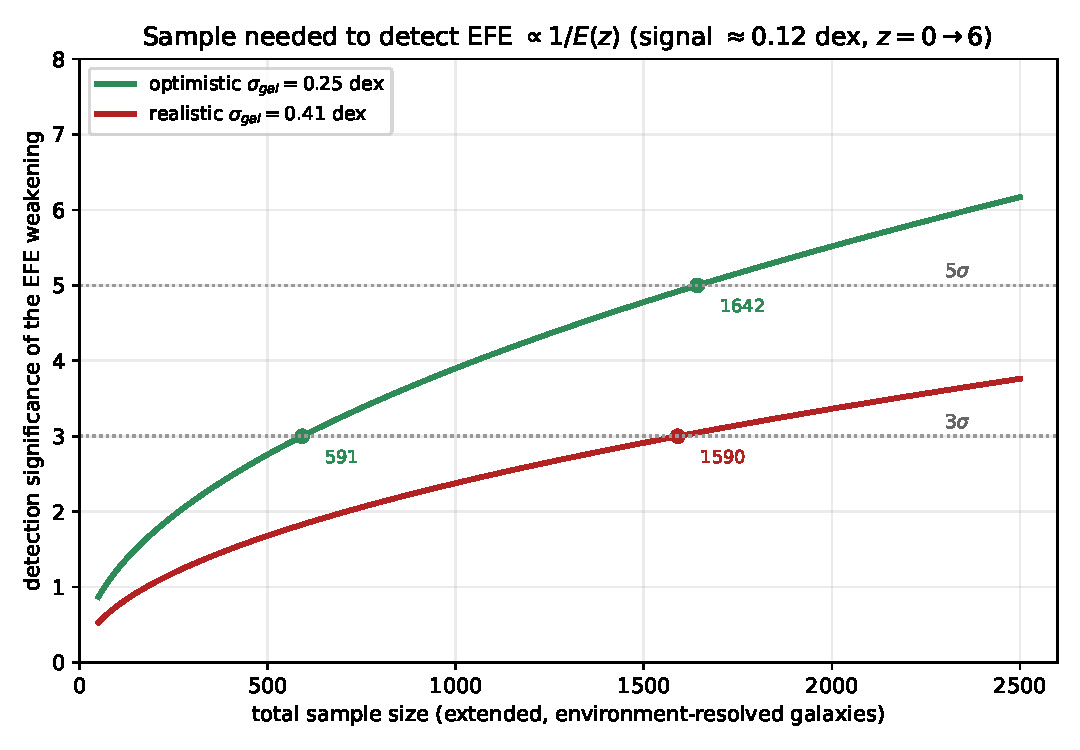
\includegraphics[width=0.74\textwidth]{efe_fig3_samplesize.pdf}
\caption{\textbf{Sample size.} Detection significance of the EFE \emph{weakening}
versus total number of extended, environment-resolved galaxies, for the realistic and
optimistic per-galaxy noise. Markers give the $3\sigma$ and $5\sigma$ samples.}
\label{fig:N}
\end{figure}

\section{The observing proposal}
The campaign is a staged, multi-facility build of a \emph{homogeneous}
$\az$-versus-environment ladder from $z=0$ to $z\gtrsim4$. Every target must satisfy
three selection criteria that are usually ignored: it must be \textbf{extended}
(internal $\gbar<\az(z)$, i.e.\ genuinely deep-MOND---compact galaxies are Newtonian
and carry no signal); it must be \textbf{environment-classified} (isolated vs.\
embedded, with $\gext$ estimated from the local density field or host); and it must
have a \textbf{full baryon census} (stars \emph{and} gas).

\begin{table}[h]
\centering
\small
\begin{tabular}{lllrl}
\hline
$z$ bin & tracer & facility & $N_{\rm tgt}$ & role \\
\hline
$0.0$ & H{\sc i}/H$\alpha$ rotation & SPARC (archival) & $\sim$175 & local anchor; RAR, EFE($z{=}0$)\\
$0.3$--$0.8$ & H$\alpha$ IFU & VLT/MUSE, KMOS & $\sim$150 & establish EFE; environment split\\
$1$--$2.5$ & H$\alpha$/Pa$\alpha$ IFU & JWST/NIRSpec & $\sim$150 & $\az$, $M_\star$, environment\\
$2.5$--$4$ & [C{\sc ii}]/CO disks & ALMA & $\sim$150 & rotation, $M_{\rm gas}$, $M_{\rm dyn}$\\
$>4$ & [C{\sc ii}]\,+\,rest-optical & ALMA\,+\,ELT/HARMONI & $\sim$150 & extended deep-MOND; the lever arm\\
\hline
\end{tabular}
\caption{A staged EFE-versus-$z$ campaign. The low-$z$ bins establish that the EFE
exists and pin systematics; the $z\gtrsim2.5$ bins, where $\Ez\gtrsim3$, carry the
discriminating power. Total $\sim$750 (optimistic floor) scaling to $\sim$1600 if the
realistic noise holds.}
\end{table}

\noindent
\textbf{Sequencing.} (1) Re-analyse SPARC and existing VLT/JWST IFU surveys
(KMOS$^{\rm 3D}$, KROSS, and JWST Cycle-1/2 kinematics) with a \emph{single} pipeline
and an environment split---this already tests level (i) and calibrates $\sigma_{\rm
gal}$. (2) A dedicated JWST+ALMA program for $1<z<4$ extended galaxies with gas
masses. (3) ELT/HARMONI and ALMA deep fields for the $z>4$ anchor. The decisive
double-difference emerges only once the $z>2.5$ bins are populated at the few-hundred
level---an ELT-era, multi-cycle effort.

\section{Caveats and degeneracies}
We state the risks plainly.
\begin{enumerate}\itemsep1pt
\item \textbf{The premise chain is long.} The test is conditional on (a) MOND being a
real description---contested by wide-binary analyses, which split between a Newtonian
preference \cite{Banik2024} and a MOND-consistent signal \cite{Chae2023}; (b) the
$\az$-scale being universal enough to define, itself debated \cite{Rodrigues2018}; and
(c) the EFE being real at $z=0$ \cite{Chae2020}. Each link is uncertain.
\item \textbf{Environments evolve.} $\gext$ is not fixed in physical units across
cosmic time; the analysis must \emph{measure} $\gext$ per galaxy (local density, host
mass) and match it across $z$, not assume it. This is a systematic, not a statistical,
limitation.
\item \textbf{Selection.} High-$z$ kinematic samples favour compact,
dispersion-supported systems that are Newtonian and signal-free; the campaign must
deliberately target extended, rotation-supported, low-acceleration galaxies.
\item \textbf{Baryon census.} Gas can dominate the high-$z$ baryon budget; without
$M_{\rm gas}$, $\gbar$ and hence the EFE offset are biased.
\end{enumerate}
None of these is fatal, but together they make this a careful, next-generation
measurement rather than a re-analysis of existing data.

\section{Conclusion}
If the Milgromian scale is cosmological, $\az=\tfrac{c}{2}\sqrt{G\rho}=cH(z)/Z$, then
the External Field Effect must fade with redshift as $\eta_0/\Ez$. This is the one
prediction of the evolving-$\az$ hypothesis that is simultaneously \emph{forbidden in
dark matter} and \emph{distinct from constant-$\az$ MOND}, and it is therefore the
cleanest available discriminator---cleaner than the direct $\az(z)$ measurement, whose
present $\sim2\sigma$ hint is $\Lambda$CDM-degenerate. The signal is small
($\sim0.1$\,dex) and the required sample large ($\sim$590--1600 extended,
environment-resolved galaxies, weighted to $z\gtrsim2$), placing a decisive test in
the JWST\,+\,ALMA\,+\,ELT next decade. A robust detection would establish two things
at once: that the equivalence principle is violated in galaxy dynamics as MOND
predicts, and that its acceleration scale is set by the expanding universe---evidence
for an emergent, cosmologically-rooted origin of inertia. A null result for the
\emph{evolution}, given a low-$z$ EFE, would falsify the cosmological reading and
return $\az$ to the status of a constant. Either way the question is decidable, and
the experiment is specified.

\paragraph{Reproducibility.} The signal, error budget, sample sizes and all three
figures are generated by \texttt{reviews/efe\_evolution\_forecast.py} and
\texttt{papers/efe\_forecast\_figures.py}; the current-data fit by
\texttt{reviews/stresstest\_piece3\_evolution.py}.

\begin{thebibliography}{99}
\small
\bibitem{Milgrom1983} M.~Milgrom, Astrophys.\ J.\ {\bf 270}, 365 (1983).
\bibitem{Famaey2012} B.~Famaey and S.~S.~McGaugh, Living Rev.\ Relativity {\bf 15}, 10 (2012).
\bibitem{McGaugh2016} S.~S.~McGaugh, F.~Lelli, and J.~M.~Schombert, Phys.\ Rev.\ Lett.\
  {\bf 117}, 201101 (2016); F.~Lelli, S.~S.~McGaugh, and J.~M.~Schombert, Astron.\ J.\
  {\bf 152}, 157 (2016).
\bibitem{Lelli2017} F.~Lelli, S.~S.~McGaugh, J.~M.~Schombert, and M.~S.~Pawlowski,
  Astrophys.\ J.\ {\bf 836}, 152 (2017).
\bibitem{Milgrom2011} M.~Milgrom, ``MOND's acceleration scale as a fundamental
  quantity,'' (2011).
\bibitem{Milgrom2014} M.~Milgrom, ``Cosmological variation of the MOND constant'' /
  ``MOND laws of galactic dynamics,'' Mon.\ Not.\ R.\ Astron.\ Soc.\ {\bf 437}, 2531 (2014).
\bibitem{BekensteinMilgrom1984} J.~Bekenstein and M.~Milgrom, Astrophys.\ J.\ {\bf 286}, 7 (1984).
\bibitem{Chae2020} K.-H.~Chae, F.~Lelli, H.~Desmond, S.~S.~McGaugh, P.~Li, and
  J.~M.~Schombert, Astrophys.\ J.\ {\bf 904}, 51 (2020).
\bibitem{Skordis2021} C.~Skordis and T.~Z\l osnik, Phys.\ Rev.\ Lett.\ {\bf 127}, 161302 (2021).
\bibitem{Verlinde2017} E.~P.~Verlinde, SciPost Phys.\ {\bf 2}, 016 (2017).
\bibitem{Tian2022} Y.~Tian \textit{et al.}, ``$\Lambda$CDM with baryons versus MOND:
  the time evolution of the RAR / apparent $a_0$,'' (2022).
\bibitem{deGraaff2024} A.~de~Graaff \textit{et al.}, JADES dynamical masses at high
  redshift (2024).
\bibitem{Banik2024} I.~Banik \textit{et al.}, Mon.\ Not.\ R.\ Astron.\ Soc.\ {\bf 527}, 4573 (2024).
\bibitem{Chae2023} K.-H.~Chae, Astrophys.\ J.\ {\bf 952}, 128 (2023).
\bibitem{Rodrigues2018} D.~C.~Rodrigues, V.~Marra, A.~del~Popolo, and D.~Davari,
  Nature Astronomy {\bf 2}, 668 (2018).
\bibitem{Varasteanu2025} V\u{a}r\u{a}\c{s}teanu \textit{et al.} (2025); intermediate-$z$
  acceleration-scale determination.
\bibitem{MUSEDARK2026} MUSE--DARK collaboration, MUSE--DARK III (2026); $z\simeq0.9$
  acceleration-scale determination.
\end{thebibliography}

\end{document}
